%----------------------------------------------------------------------
%	DIRC@EIC CHAPTER
%----------------------------------------------------------------------
\label{ch:eicdirc}
The BaBar DIRC was able to reach a performance of 3 standard deviations (s.d.) separation for pions and kaons at up to 4 GeV/c particle momentum. The PANDA Barrel DIRC wishes to achieve similar performance, but due to space constraints they will be using a smaller expansion volume and must therefore rely on optical focusing of the Cherenkov photons to reach this performance. In both cases the separation power requires a per track Cherenkov angle resolution (Eq. \ref{eq:performance}) of 2.5 mrad The physics goals of an EIC require a pion/kaon separation of 3 s.d. at up to 6 GeV/c momentum, which requires 1 mrad track Cherenkov angle resolution. The graph in Figure \ref{fig:PID_performance} shows pion-kaon separation as a function of particle momentum for different assumptions of the per track Cherenkov angle resolution, highlighting the achieved performance of BaBar and the desired performance of PANDA and EIC. In order to reach this high resolution in a compact space the EIC DIRC must incorporate cutting-edge technology in focusing optics and photo sensor granularity and timing resolution.

\begin{figure}[!htb]
	\centering
	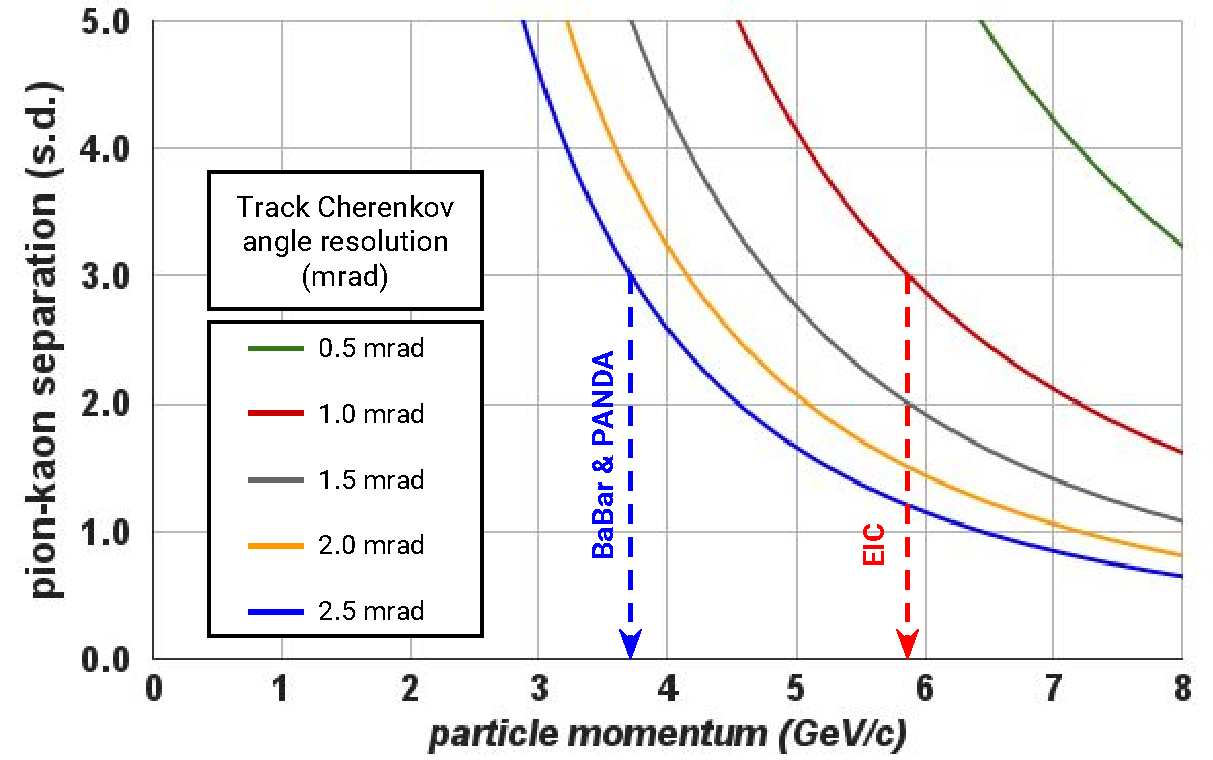
\includegraphics[width=\textwidth]{PID_performance.pdf}
	\caption{Pion-kaon separation as a function of particle momentum for different assumptions of the per track Cherenkov angle resolution. The PID requirements of the EIC necessitate a per track resolution of 1 mrad, while BaBar and PANDA needed only 2.5 mrad resolution.}
	\label{fig:PID_performance}
\end{figure}

%----------------------------------------------------------------------
%	CURRENT BASELINE DESIGN SECTION
%----------------------------------------------------------------------
\section{High-Performance DIRC Components and Design}
The baseline design of a DIRC for EIC has been constructed in a GEANT4 simulation based on that of the PANDA prototype DIRC, as shown in Figure \ref{fig:baseline_design}. There are 16 modules, called bar boxes, each containing 11 radiator bars 4200 mm long with a cross section of $17\times35.4\unit{mm}^2$. The 16 bar boxes are arranged in a barrel with a radius of 1 m around the beam line. Mirrors are coupled to one end of each bar, and a special 3-layer lens, discussed in more detail later, is attached to the other end. The lens is then coupled directly to a prism-shaped expansion volume made of fused silica, the same material as the radiator bars. The prism has an opening angle of $38^\circ$ with dimensions of $284.3\times390\times300\unit{mm}^3$. The $284.3\times390\unit{mm}^2$ detector plane of each prism is covered with micro-channel plate photomultiplier tubes (MCP-PMTs) with 27,690 $2\times2\unit{mm}^2$ pixels, for a total of 443,040 channels across the entire detector to record the location and arrival time of each detected Cherenkov photon. The dependence of the performance on the granularity of the detectors is shown later in this chapter.

\begin{figure}[!htb]
	\centering
	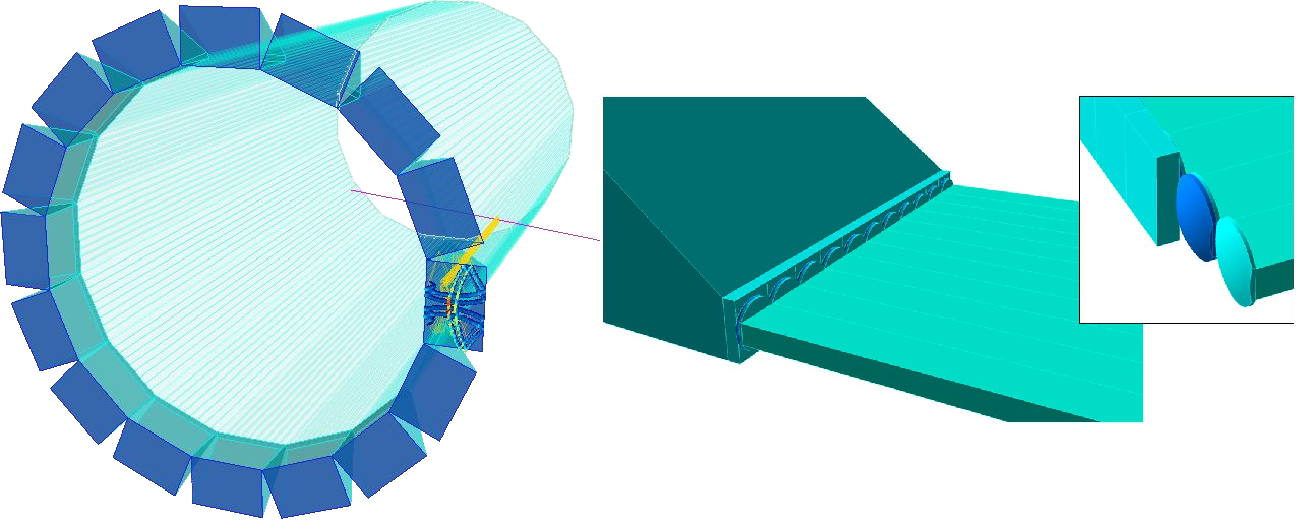
\includegraphics[width=\textwidth]{EIC_DIRC_baseline.pdf}
	\caption{Left: full GEANT4 simulation of the current DIRC at EIC baseline design with 16 bar boxes, 176 radiator bars, a 3-layer lens focusing optic, and a $38^\circ$ prism expansion volume. Right: a zoom in on a single bar box and the layering of the lens.}
	\label{fig:baseline_design}
\end{figure}

%----------------------------------------------------------------------
%----------------------------------------------------------------------
\subsection{Focusing Optics}

\begin{figure}[!htb]
	\centering
	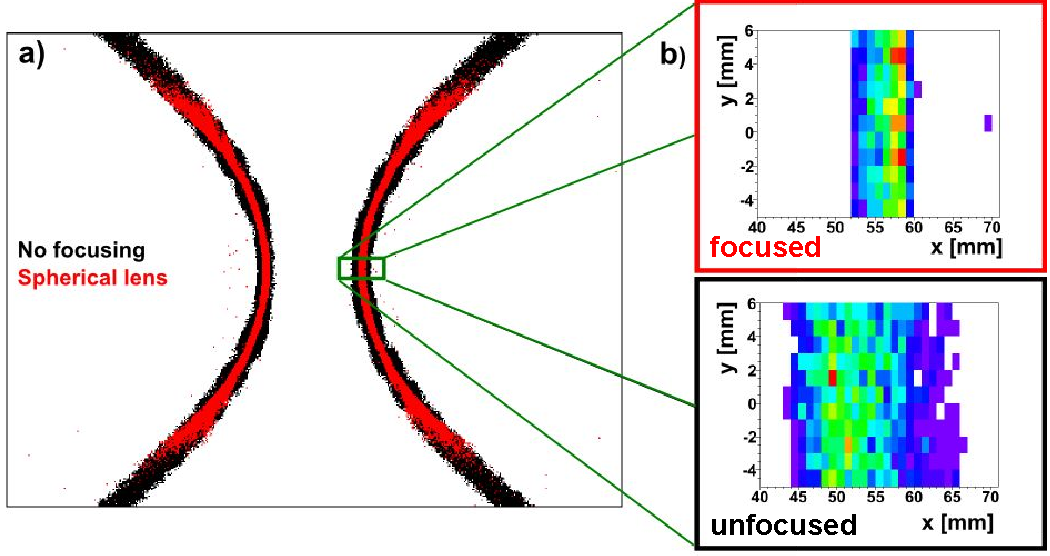
\includegraphics[width=\textwidth]{airgap_dispersion.pdf}
	\caption[Simulated hit pattern of PANDA DIRC without (black) and with (red) air gap lens focusing (a). On the outer edges of the ring image the lens is becoming dispersive  and losing photons, while near the center of the rings the lens does a good job of focusing the image, as seen more clearly in b).]{Simulated hit pattern of PANDA DIRC without (black) and with (red) air gap lens focusing (a) \cite{GregThesis}. On the outer edges of the ring image the lens is becoming dispersive  and losing photons, while near the center of the rings the lens does a good job of focusing the image, as seen more clearly in b).}
	\label{fig:airgap_dispersion}
\end{figure}

The pixel and bar size of a DIRC detector are important contributions to the Cherenkov angle resolution for small expansion volumes. The influence of the bar size can, however, be offset by focusing the Cherenkov photons. The FDIRC R\&D program first developed the concept of using focusing mirrors for DIRC detectors. The PANDA Barrel DIRC group settled on using a focusing lens between the radiator bar and the expansion volume. A standard lens made of fused silica with an air gap between the lens and the expansion volume was first studied. However, the focal plane of a single lens is highly parabolic in shape. Figure \ref{fig:airgap_dispersion} shows that while an air gap lens provides good focusing of the Cherenkov pattern in the central region of the ring, where photons are more or less perpendicular to the lens, it becomes defocused nearer to the edges of the pattern and loses photons. This deterioration of the image quality for steeper angles is a combination of lens aberrations, the curved focal plane, and the so-called kaleidoscopic effect \cite{FDIRCMathematica}.

A 2-layer compound lens composed of fused silica and a layer of high-refractive index material Lanthanum crown glass (NLaK33) \cite{SchottData}, $n \approx 1.75$, was also studied. This design couples directly to the expansion volume, greatly reducing the loss of photons at steeper angles. Figure \ref{fig:lens_photon_yield} shows a comparison of the photon yield from a bar radiator with no focusing (green), a standard air gap lens (red), and a 2-layer lens (blue) for two cases. In the $125^\circ$ case (left) both lenses have comparable photon yields, because the angle between the photons and the lens is fairly shallow. In the $90^\circ$ case (right), however, the photon yield for the air gap lens is dramatically lowered due to the steep angles between the photons and the lens. The photon yield for the no focusing option is quite deceiving in that it produces a much higher average photon yield than either lens, but the reconstruction of the Cherenkov angle is nearly impossible to within a reasonable measure for the perpendicular case.

\begin{figure}[!htb]
	\centering
	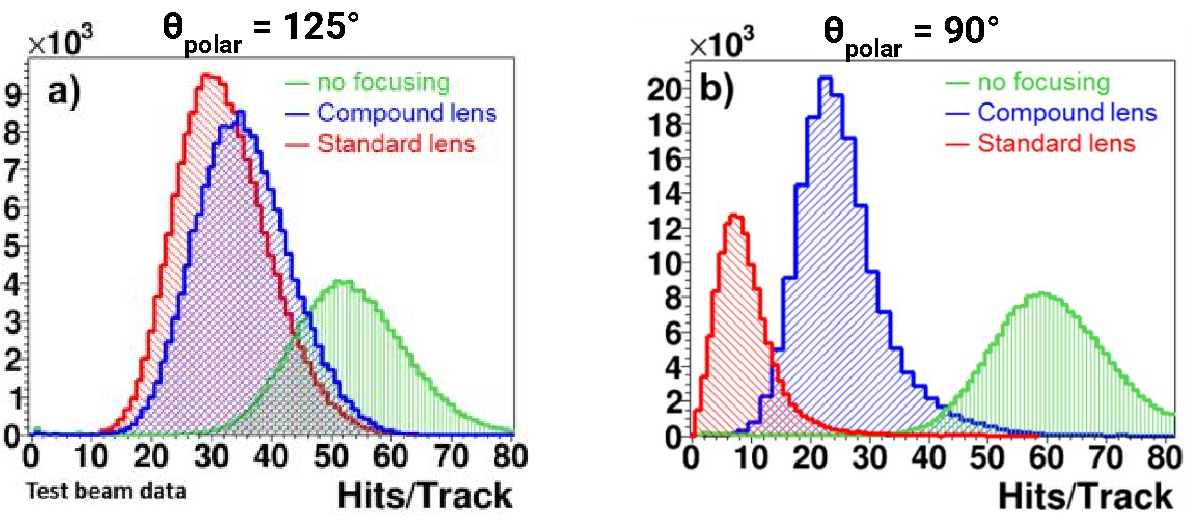
\includegraphics[width=\textwidth]{lens_photon_yield_comparison.pdf}
	\caption[Comparison of the photon yield per track for a DIRC bar with no focusing (green), a standard air gap lens (red), and a 2-layer compound lens (blue) for polar angles of $125^\circ$ (left) and $90^\circ$ (right) \cite{GregThesis}. The standard and compound lenses have comparable yields at $125^\circ$, but the standard lens clearly loses a large amount of photons in the perpendicular case.]{Comparison of the photon yield per track for a DIRC bar with no focusing (green), a standard air gap lens (red), and a 2-layer compound lens (blue) for polar angles of $125^\circ$ (left) and $90^\circ$ (right). The standard and compound lenses have comparable yields at $125^\circ$, but the standard lens clearly loses a large amount of photons in the perpendicular case.}
	\label{fig:lens_photon_yield}
\end{figure}

The 2-layer lens design solves the problem of photon yield loss from the air gap lens at steeper angles and will allow the PANDA Barrel DIRC to reach their desired separation power. However, as discussed earlier, this separation power of 3 s.d. at 4 GeV/c is insufficient for the requirements of a DIRC at EIC. The key to solving this problem was in designing a special 3-layer spherical compound lens. The advantage of this 3-layer lens design over a traditional optical lens or the 2-layer lens is the shape of the focal plane. According to simulation the focal plane of the 3-layer lens is relatively flat, as shown in Figure \ref{fig:lens_focal_plane}. Photos of a prototype lens tested at CERN in 2015 and an exploded view of the lens layers and dimensions are shown in Figure \ref{fig:3CS_schematic}. It contains a layer of NLaK33 sandwiched between two layers of fused silica. The two radii of the middle layer were optimized to remove aberrations present in standard lenses by first defocusing and then refocusing transmitted photons to create a flat focal plane, matching the geometry of the prism expansion volume. Five prototype lenses were produced for evaluating the performance of the lens design in a test beam, for measuring the radiation hardness of the NLaK33 material, and for evaluating the focal plane. These tests will be discussed in greater detail in Chapters \ref{ch:components} and \ref{ch:analysis}.

\begin{figure}[!htb]
	\centering
	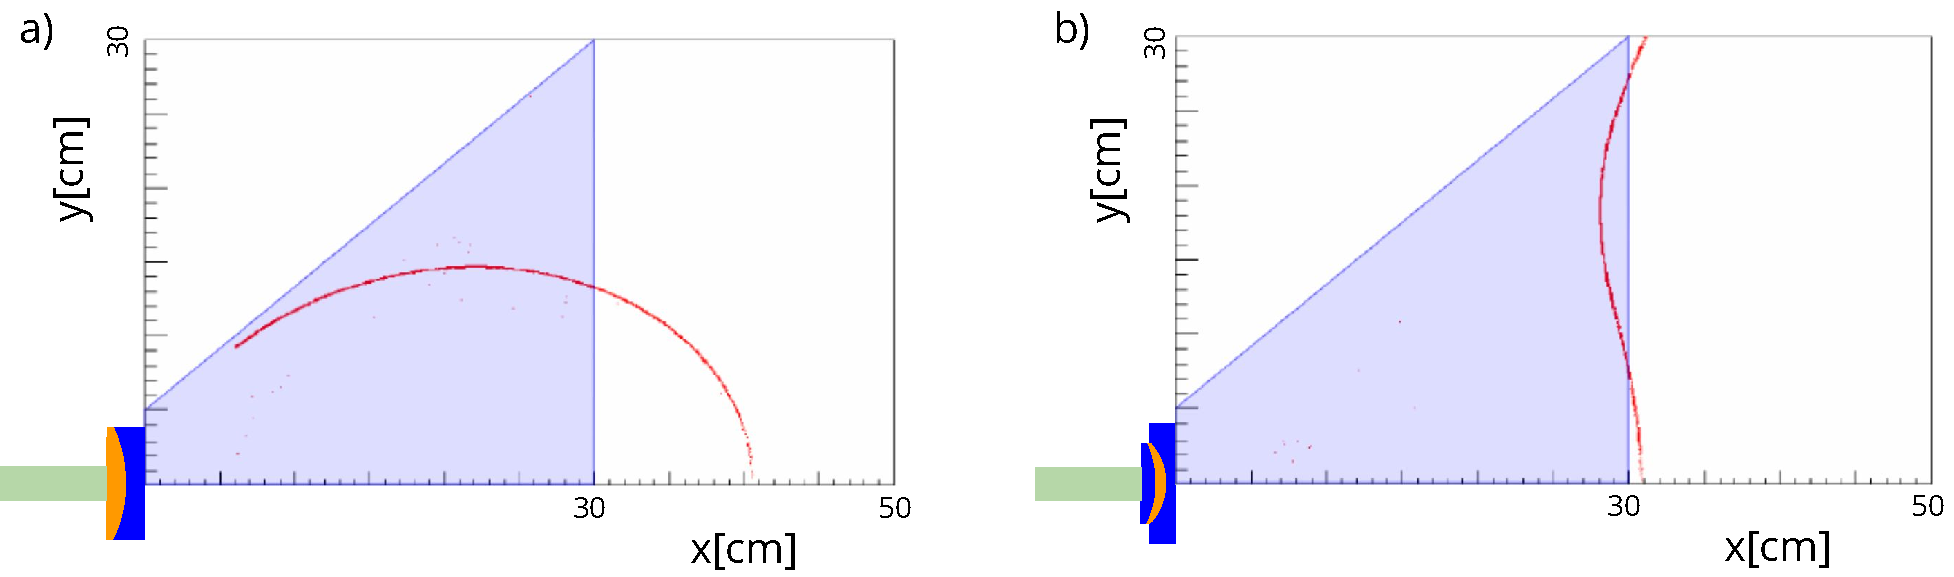
\includegraphics[width=\textwidth]{lens_comparison}
	\caption{The simulated focal planes (red lines) of a 2-layer lens (left) and the 3-layer lens (right) compared to the shape of the expansion volume prism (grey). Obviously the focal plane of the 2-layer lens is highly parabolic in shape, whereas the 3-layer lens focal plane is relatively flat, allowing for a better resolution of the Cherenkov angle.}
	\label{fig:lens_focal_plane}
\end{figure}

\begin{figure}[!htb]
	\centering
	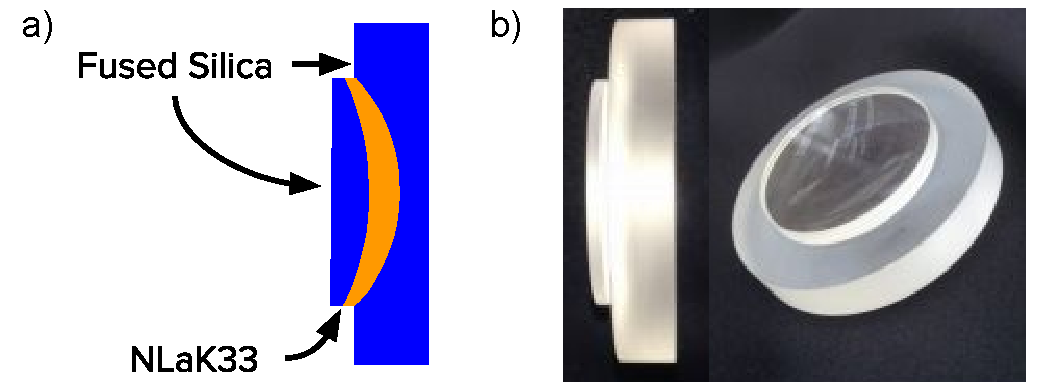
\includegraphics[scale=0.7]{3CS_schematic.pdf}
	\caption{Prototype 3-layer lens built for optical testing (a), and an exploded view of each layer with dimensions (b).}
	\label{fig:3CS_schematic}
\end{figure}

%----------------------------------------------------------------------
%----------------------------------------------------------------------
%\subsection{Sensors}

%----------------------------------------------------------------------
%	SIMULATION SECTION
%----------------------------------------------------------------------
\clearpage
\section{Simulated Performance}

\subsection{Geometric Reconstruction}
Simulated reconstructions of the Cherenkov angle for kaons and pions at 6 GeV/c with a $125^{\circ}$ polar angle using the design parameters above are shown in Figure \ref{fig:EIC_reconstruction}. The signal is very clean and the mean and SPR of the distribution are easily extracted. Figure \ref{fig:EIC_performance}a shows the photon yield, or multiplicity, per polar angle for fifty 6 GeV/c pions, and Figure \ref{fig:EIC_performance}b shows the Single Photon Resolution (SPR) \footnote{Three points are normally required to define a circle and thus extract a radius. However, with a perfect RICH detector it is sufficient to know only a single point on the ring as one also knows the center of the circle (i.e. the particle track). Here, too, it is sensible to talk about the resolution of single photon events as the center of the ``circle" for a DIRC (i.e. the polar angle) is known from tracking.} per polar angle for fifty 6 GeV/c kaons (red) and pions (blue). The per track Cherenkov angle resolution, given by Eq. (\ref{eq:performance}), is shown in Figure \ref{fig:EIC_track_res} for assumptions of 0.25 mrad (black), 0.5 mrad (red), 0.75 (green), and 1 mrad (blue) correlated term contributions with 6 GeV/c pions \footnote{NB: the per track Cherenkov angle resolution will be slightly different for each particle species, however, because the SPR for each particle is almost identical, showing only the results for pions is sufficient.}.  The simulations were done assuming that the sides of the 3-layer lens focusing optic were not reflective, therefore reducing the photon yield and making the performance slightly worse.

The SPR of the reconstructed Cherenkov angle was found to scale with the pixel size of the MCP-PMTs roughly as $SPR \approx SPR_{0}\sqrt{1+size^2/a^2}$, as shown in Figure \ref{fig:EIC_sensor_scaling}. Clearly the 4 mm pixel size, though not ideal, is comparable in performance to the 2 mm pixel size. This is an important factor to consider in the final design due to the increase of the cost per pixel of MCP-PMTs and with the electronics readout per channel as the size of the pixels decreases.


\begin{figure}[!htb]
	\centering
	\includegraphics[width=\textwidth]{{EIC_theta_K+_125.00}.png}
	\includegraphics[width=\textwidth]{{EIC_theta_pi+_125.00}.png}
	\caption{Reconstructed $\thetaC$ spectrum for 6 GeV/c kaons (top) and pions (bottom) and a $125^{\circ}$ polar angle.}
	\label{fig:EIC_reconstruction}
\end{figure}

\begin{figure}[!htb]
	\centering
	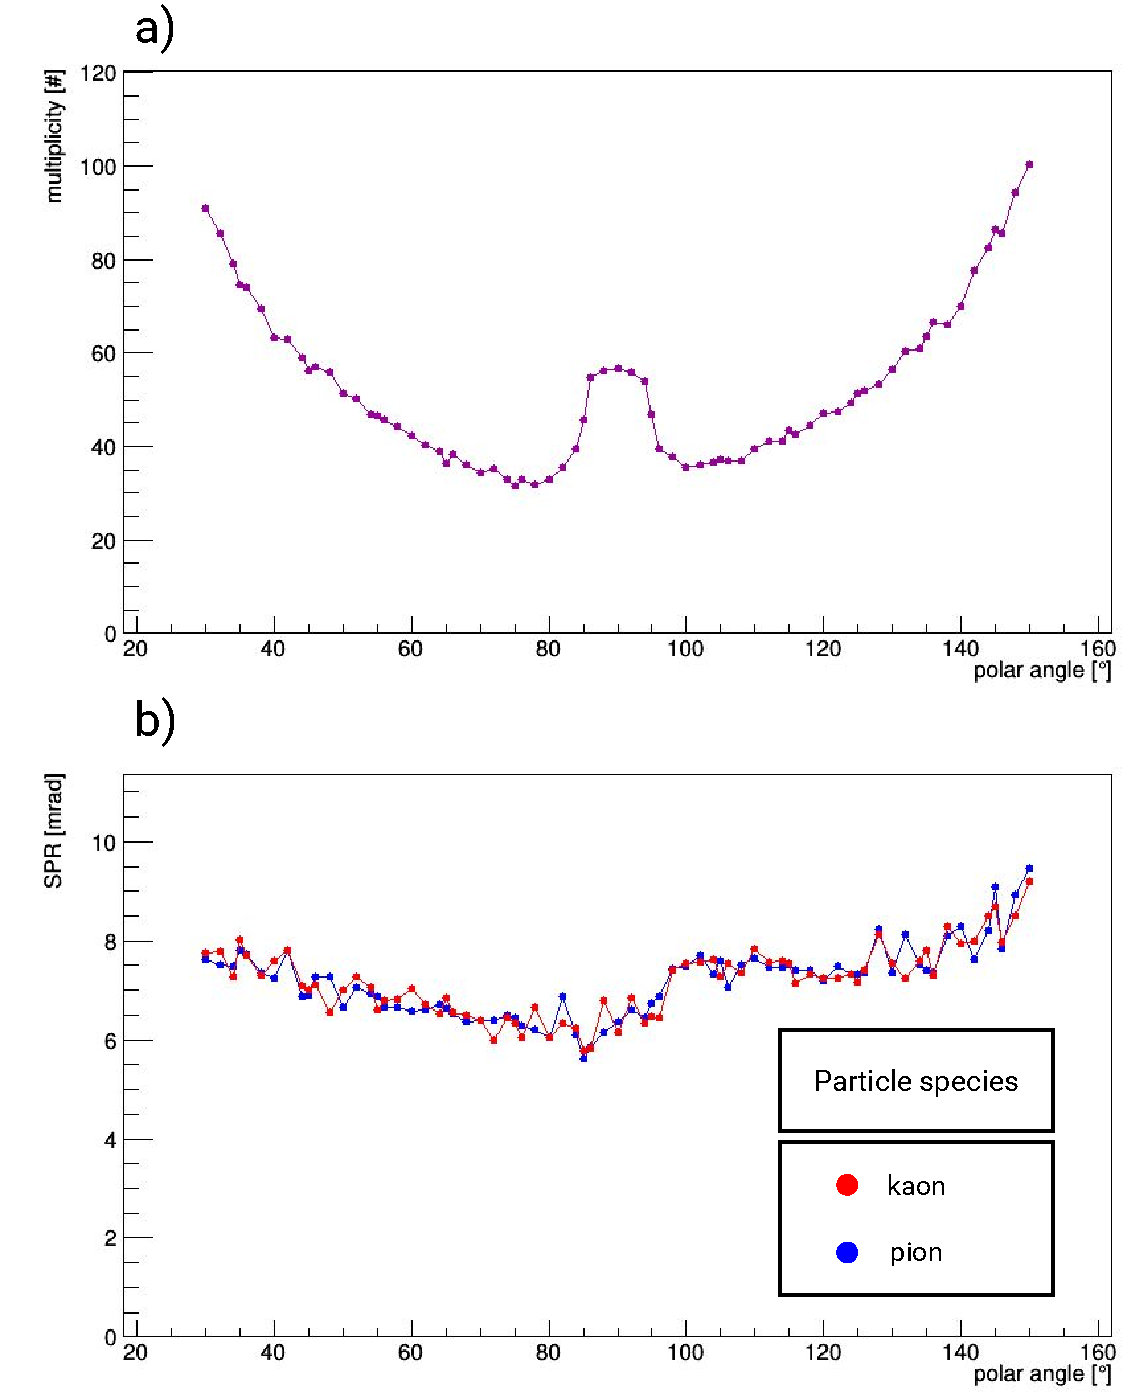
\includegraphics[width=\textwidth]{EIC_performance.pdf}
	\caption{The multiplicity (a) and SPR (b) performance per polar angle of the EIC DIRC baseline design. Plots were generated using fifty particles (kaons in red, pions in blue) at 6 GeV/c per polar angle.}
	\label{fig:EIC_performance}
\end{figure}

\begin{figure}[!htb]
	\centering
	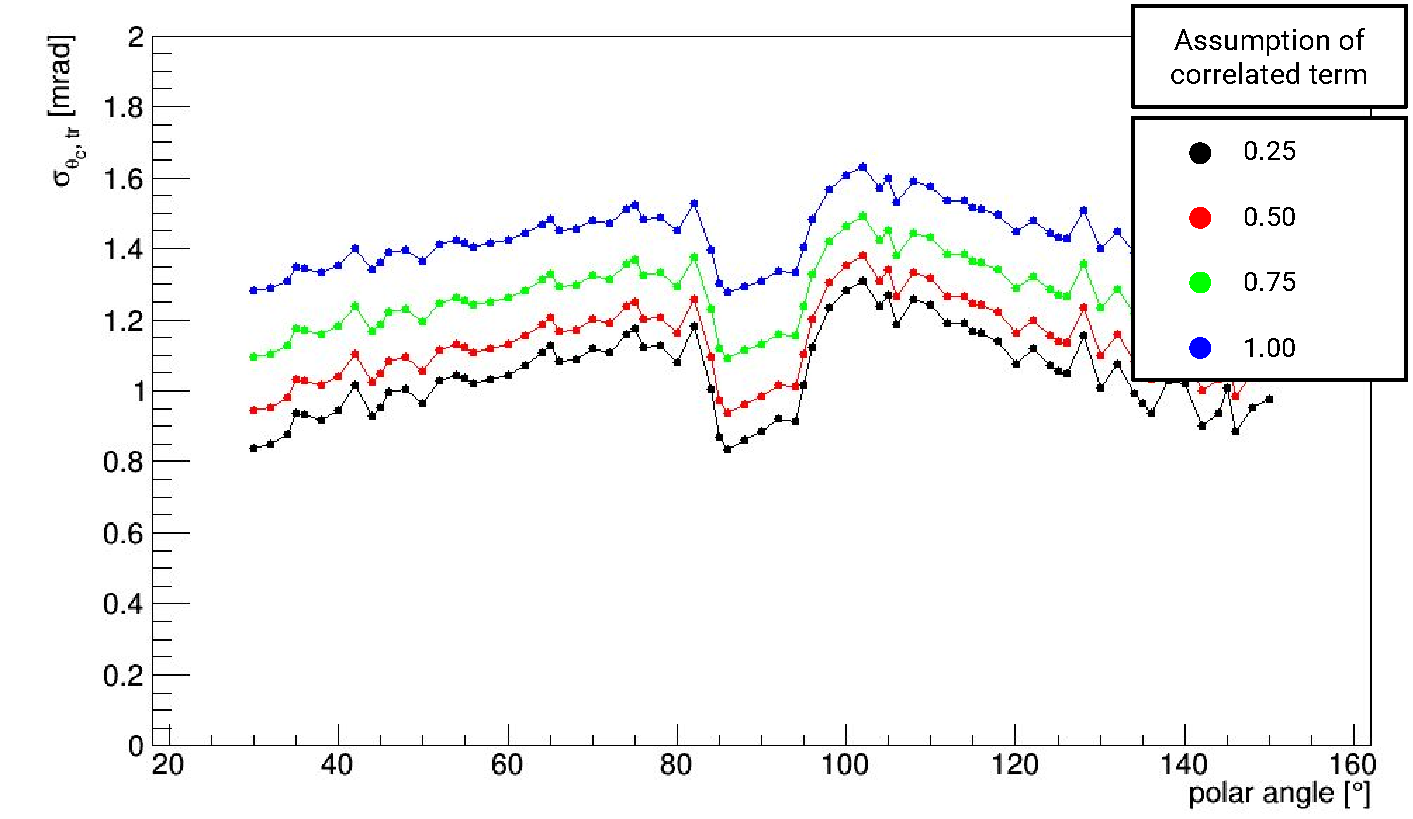
\includegraphics[width=\textwidth]{EIC_track_res.pdf}
	\caption{The per track Cherenkov angle resolution of the EIC DIRC with different assumptions of the correlated term, $\sigma_{correlated}$: 0.25 mrad (black), 0.5 mrad (red), 0.75 (green), and 1 mrad (blue).}
	\label{fig:EIC_track_res}
\end{figure}

\begin{figure}[!htb]
	\centering
	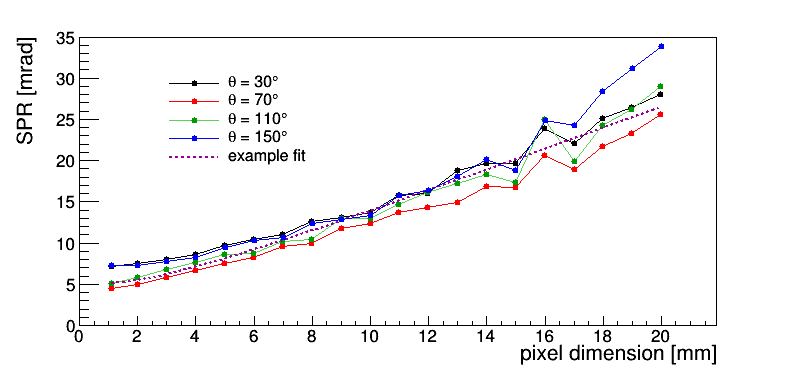
\includegraphics[width=\textwidth]{EIC_SPR_vs_sensorDim3.png}
	\caption{Scaling of the SPR as a function of the MCP-PMT pixel dimension for $30^\circ$ (black), $70^\circ$ (red), $110^\circ$ (green), and $150^\circ$ (blue) polar angle along with an example fit (dashed purple) showing that the dependence of the performance scales roughly as $\sqrt{1+\frac{pixel^2}{a^2}}$}
	\label{fig:EIC_sensor_scaling}
\end{figure}

\subsection{Time-based Reconstruction}
The methods for time-based reconstruction, as described in Chapter \ref{ch:dirc}, were also implemented for the EIC DIRC: 60,000 pions and kaons were simulated in GEANT4 using the current EIC DIRC design geometry and PDFs were generated for each detector pixel; the PDFs were then used to produce log-likelihood separation for each particle hypothesis. Figure \ref{fig:EIC_timebased_ex} shows the log-likelihood separation for pions and kaons at polar angle of $30^\circ$.  Figure \ref{fig:EIC_timebased_performance} shows the separation power (top) and the PID efficiency/mis-identification over all polar angles.

\begin{figure}[!htb]
	\centering
	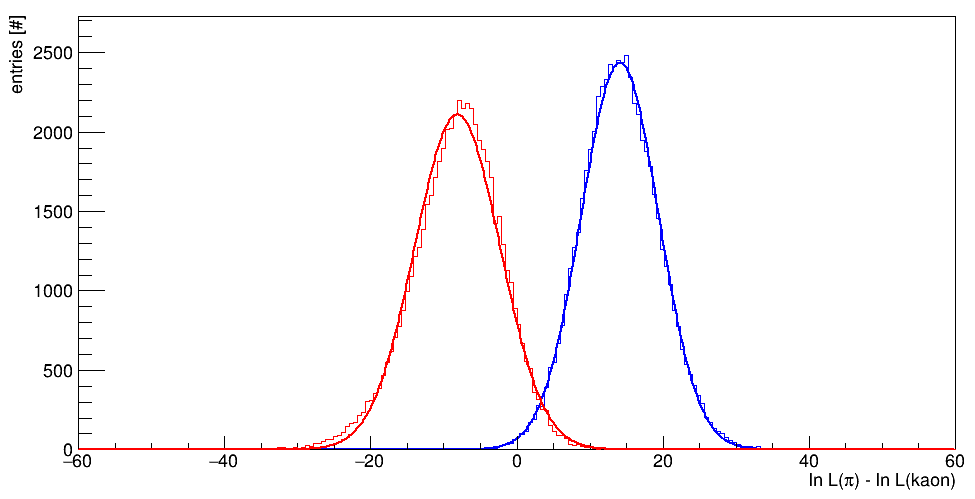
\includegraphics[width=\textwidth]{EIC_30deg_timebased_sep.png}
	\caption{Example of log-likelihood separation for pions (red) and kaons (blue) at $30^\circ$ polar angle using time-based reconstruction.}
	\label{fig:EIC_timebased_ex}
\end{figure}

\begin{figure}[!htb]
	\centering
	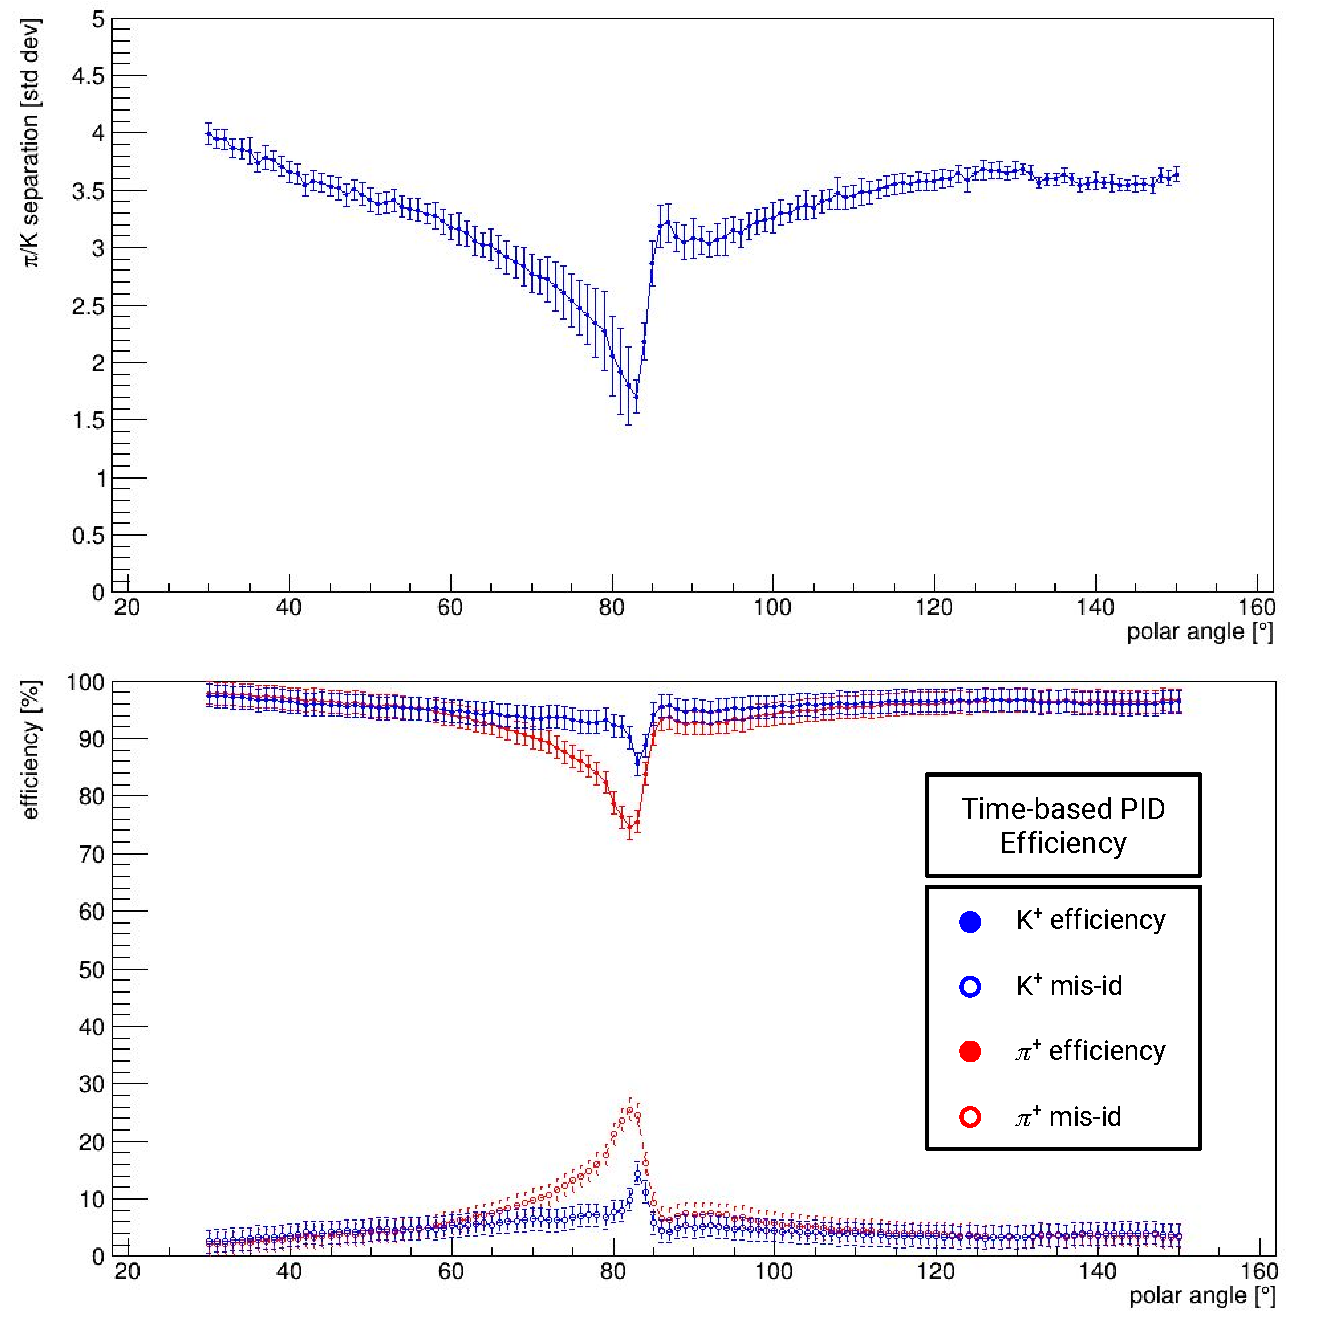
\includegraphics[width=\textwidth]{EIC_timebased_performance.pdf}
	\caption{Top: Separation power as a function of polar angle for 6 GeV/c pions and kaons using time-based reconstruction. Bottom: Efficiency (solid circles) of PID as a function of polar angle for pions (red) and kaons (blue) along with the mis-identification rate (open circles).}
	\label{fig:EIC_timebased_performance}
\end{figure}

Overall the results for both geometric and time-based reconstruction show that due to the design's large expansion volume, small pixel size, and ease of signal reconstruction the performance of this design can reach the desired performance for the required physics.
%----------------------------------------------------------------------
%	DESIGN OPTIMIZATIONS SECTION
%----------------------------------------------------------------------
%\section{Potential Optimizations}
